\documentclass[10pt]{beamer}
\usepackage{graphicx}
\usepackage{adjustbox}
\usepackage{hyperref}
\usepackage{amsmath}
\usepackage{hyperref}
\usepackage{graphicx}
\usepackage{float}
\usepackage{caption}
\usepackage{listings}
\usepackage{xcolor}
\usepackage{multimedia}


\colorlet{punct}{red!60!black}
\definecolor{background}{RGB}{240, 248, 255}
\definecolor{delim}{RGB}{20,105,176}
\colorlet{numb}{magenta!60!black}

\lstdefinelanguage{json}{
    basicstyle=\ttfamily\footnotesize\color{black},
    numbers=left,
    numberstyle=\scriptsize,
    stepnumber=1,
    numbersep=8pt,
    showstringspaces=false,
    breaklines=true,
    frame=lines,
    backgroundcolor=\color{background},
    literate=
     *{0}{{{\color{numb}0}}}{1}
      {1}{{{\color{numb}1}}}{1}
      {2}{{{\color{numb}2}}}{1}
      {3}{{{\color{numb}3}}}{1}
      {4}{{{\color{numb}4}}}{1}
      {5}{{{\color{numb}5}}}{1}
      {6}{{{\color{numb}6}}}{1}
      {7}{{{\color{numb}7}}}{1}
      {8}{{{\color{numb}8}}}{1}
      {9}{{{\color{numb}9}}}{1}
      {:}{{{\color{punct}{:}}}}{1}
      {,}{{{\color{punct}{,}}}}{1}
      {\{}{{{\color{delim}{\{}}}}{1}
      {\}}{{{\color{delim}{\}}}}}{1}
      {[}{{{\color{delim}{[}}}}{1}
      {]}{{{\color{delim}{]}}}}{1},
}

\lstset{frame=single, showstringspaces=false, columns=fixed, basicstyle={\ttfamily}, commentstyle={\it}, numbers=left, tabsize=4}

\definecolor{codebackground}{RGB}{240, 248, 255}
\definecolor{codecomment}{RGB}{106,153,85}
\definecolor{codekeyword}{RGB}{30,30,255}
\definecolor{codestring}{RGB}{163,21,21}
\definecolor{codenumber}{RGB}{100,100,100}

\lstdefinestyle{modernstyle}{
    backgroundcolor=\color{codebackground},
    commentstyle=\color{codecomment},
    keywordstyle=\color{codekeyword},
    numberstyle=\tiny\color{codenumber},
    stringstyle=\color{codestring},
    basicstyle=\ttfamily\footnotesize\color{black},
    breakatwhitespace=false,
    breaklines=true,
    captionpos=b,
    keepspaces=true,
    numbers=left,
    numbersep=5pt,
    showspaces=false,
    showstringspaces=false,
    showtabs=false,
    tabsize=4
}

\lstset{style=modernstyle}

\usetheme{Copenhagen}
\usecolortheme{default}
\setbeamertemplate{navigation symbols}{}

\title[ExaMA WP1 Vegetation]{
  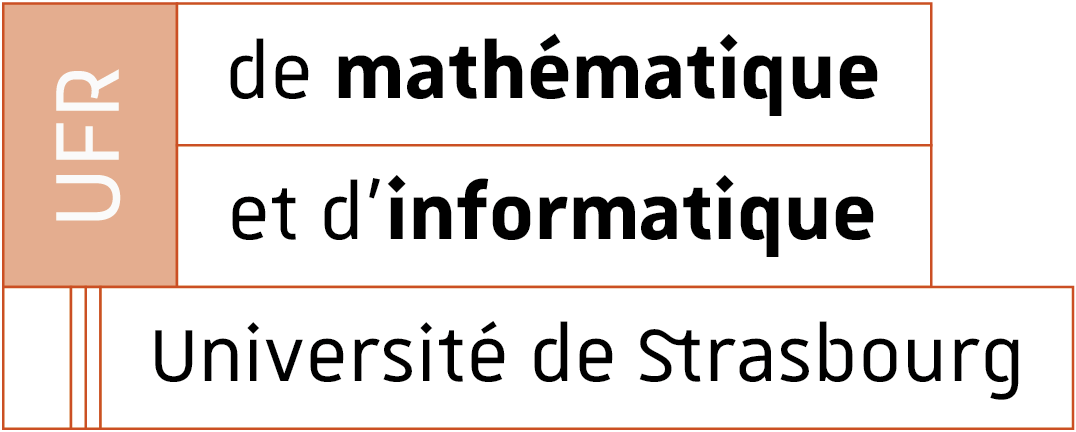
\includegraphics[width=0.8\textwidth]{images/logo-ufr.png}
  ExaMA WP1 - Vegetation}
\author[PA Senger]{Pierre-Antoine SENGER}

\begin{document}


\begin{frame}[plain]
    \begin{center}
    \begin{tabular}{c c c}
    
\includegraphics[width=100px]{images/logo-irma.png} &
    
\includegraphics[width=100px]{images/logo-inria.png} &
    
\includegraphics[width=100px]{images/logo-hidalgo2.png} \\
    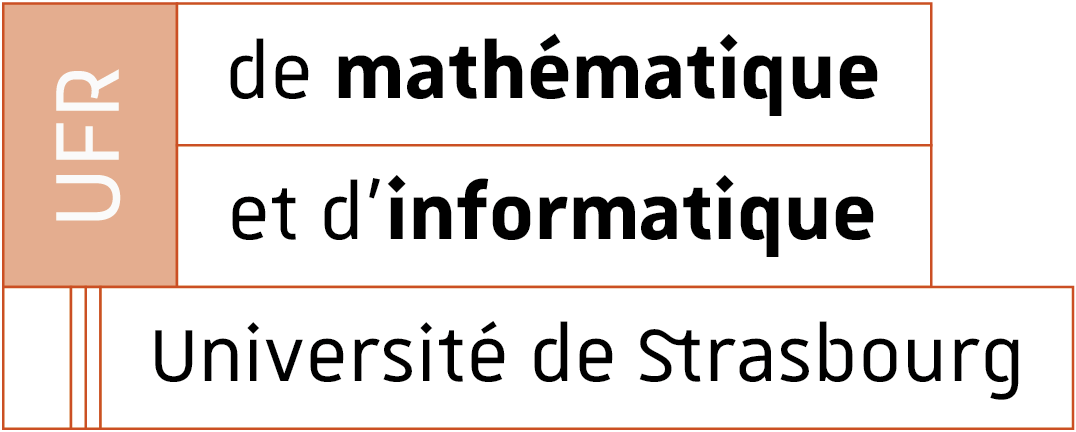
\includegraphics[width=100px]{images/logo-ufr.png} &
    
\includegraphics[width=100px]{images/logo-cemosis.png} &
    
\includegraphics[width=100px]{images/logo-numpex.png} \\
    \end{tabular}
    \end{center}
\end{frame}

\begin{frame}{Introduction}
  \titlepage
\end{frame}

\begin{frame}{Introduction}

	This project is part of a series conducted within the \textbf{exaMA} project,
	which is a segment of the \textbf{Numpex} project section.

	\begin{itemize}
		\item Exa-MA WP1 - Vegetation
		\item Exa-MA WP1 - Terrain
		\item Exa-MA WP1 - Urban Building LOD-1
		\item Exa-MA WP1 - Urban Building LOD-2 and Kinetic
		\item Exa-MA WP1 - Performance and Scalability
	\end{itemize}
\end{frame}

\begin{frame}{Context}
\begin{figure}[h]
    \centering
    \begin{minipage}{0.49\textwidth}
        \centering
        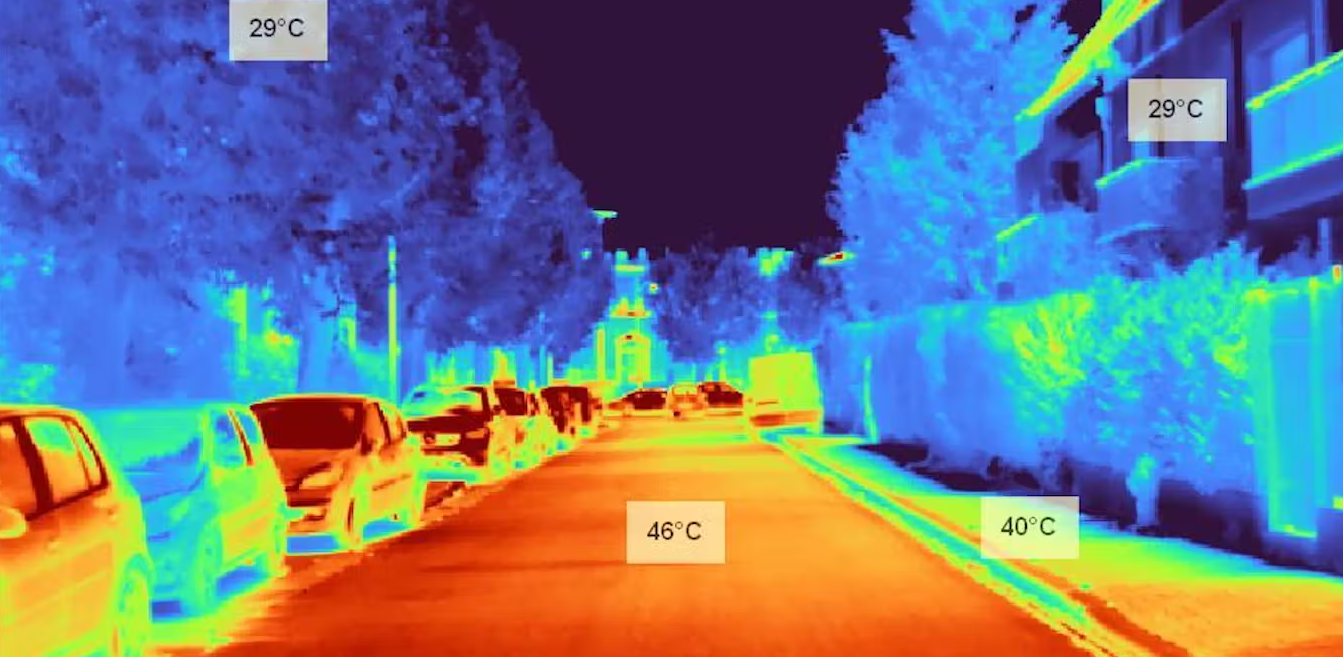
\includegraphics[width=\textwidth]{images/heat-street.png}
        \caption{Thermal image of a street depicting heat distribution}
        \label{fig:figure1}
    \end{minipage}\hfill
    \begin{minipage}{0.49\textwidth}
        \centering
        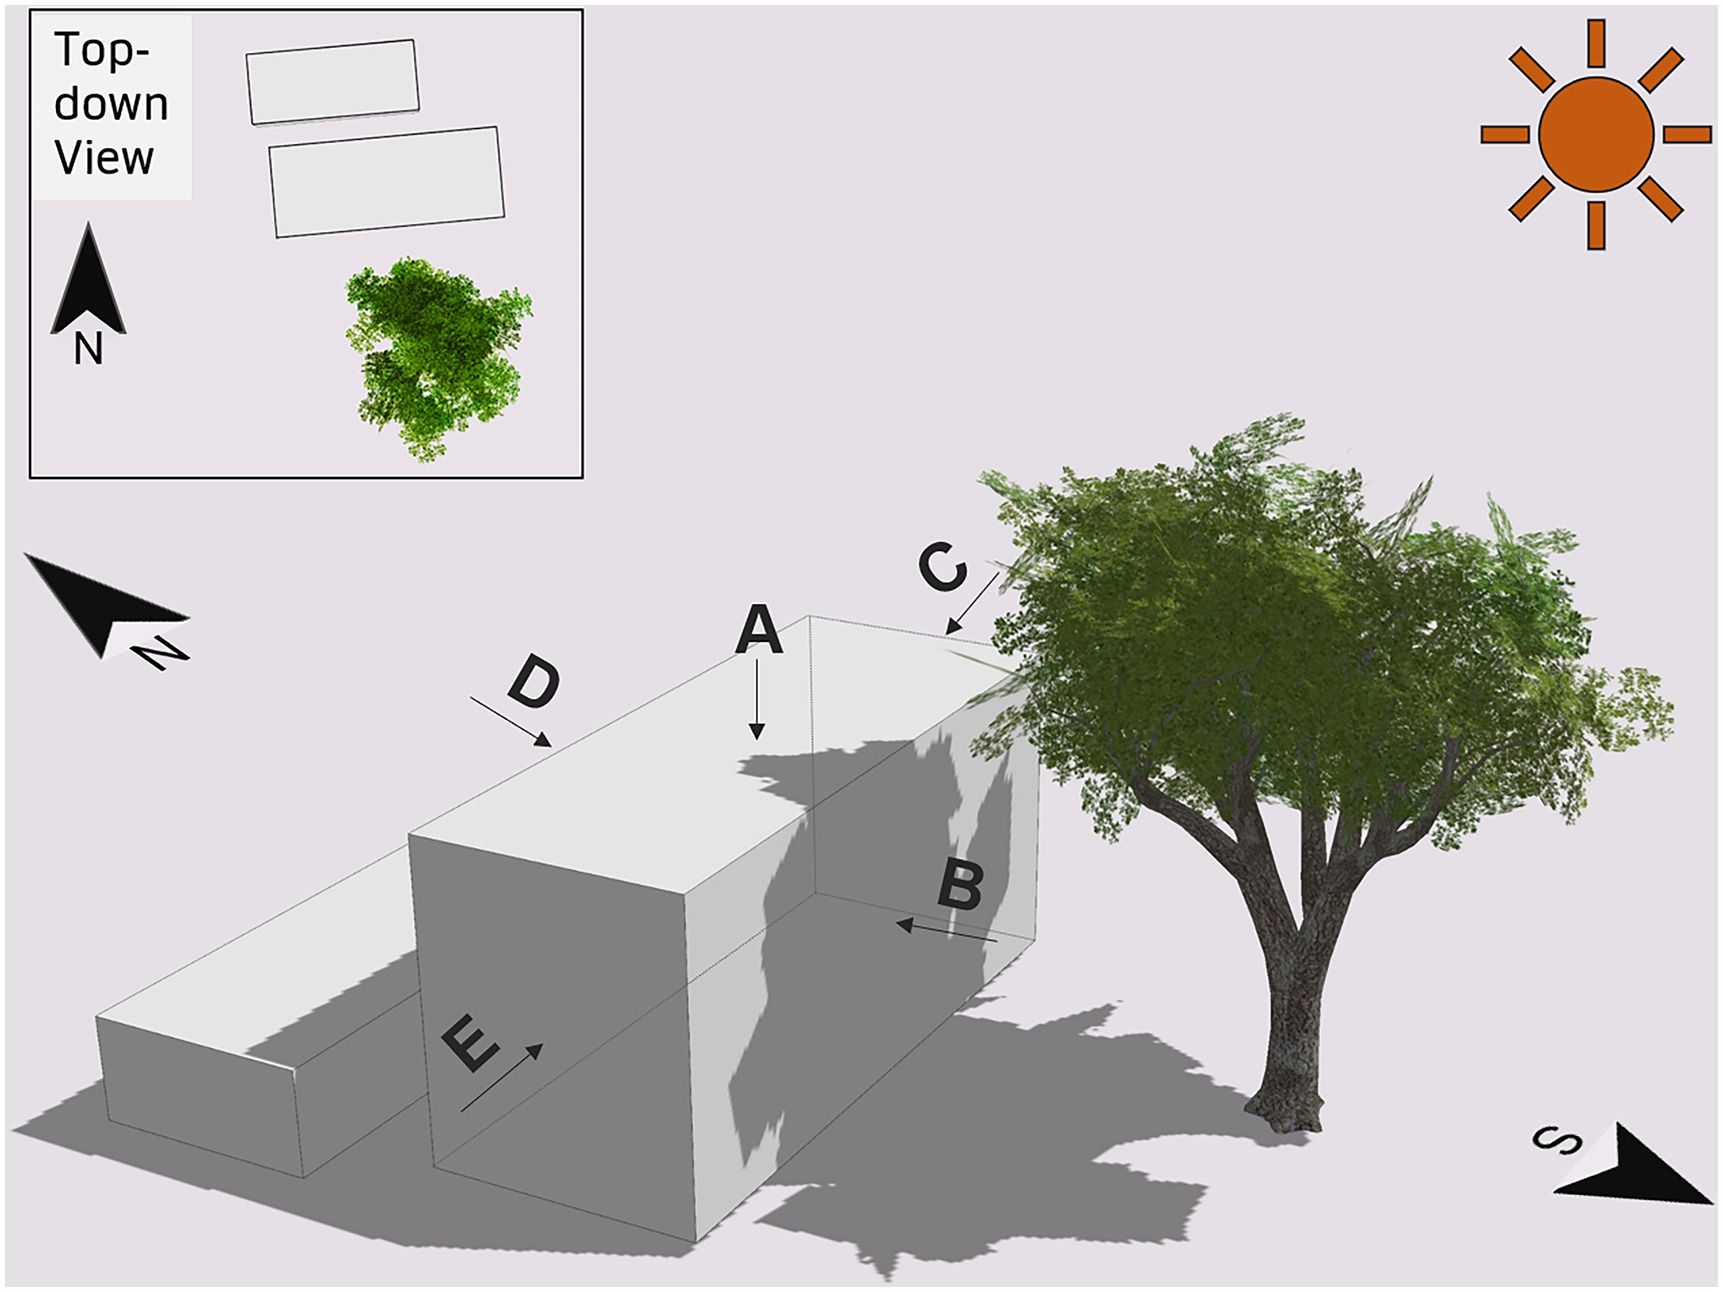
\includegraphics[width=\textwidth]{images/tree-shade.png}
        \caption{Tree providing shade to a building}
        \label{fig:figure2}
    \end{minipage}
    % \caption{Overall caption for both figures}
\end{figure}
\end{frame}

\begin{frame}{Context: Primiray focus}
	\begin{figure}
		\centering
		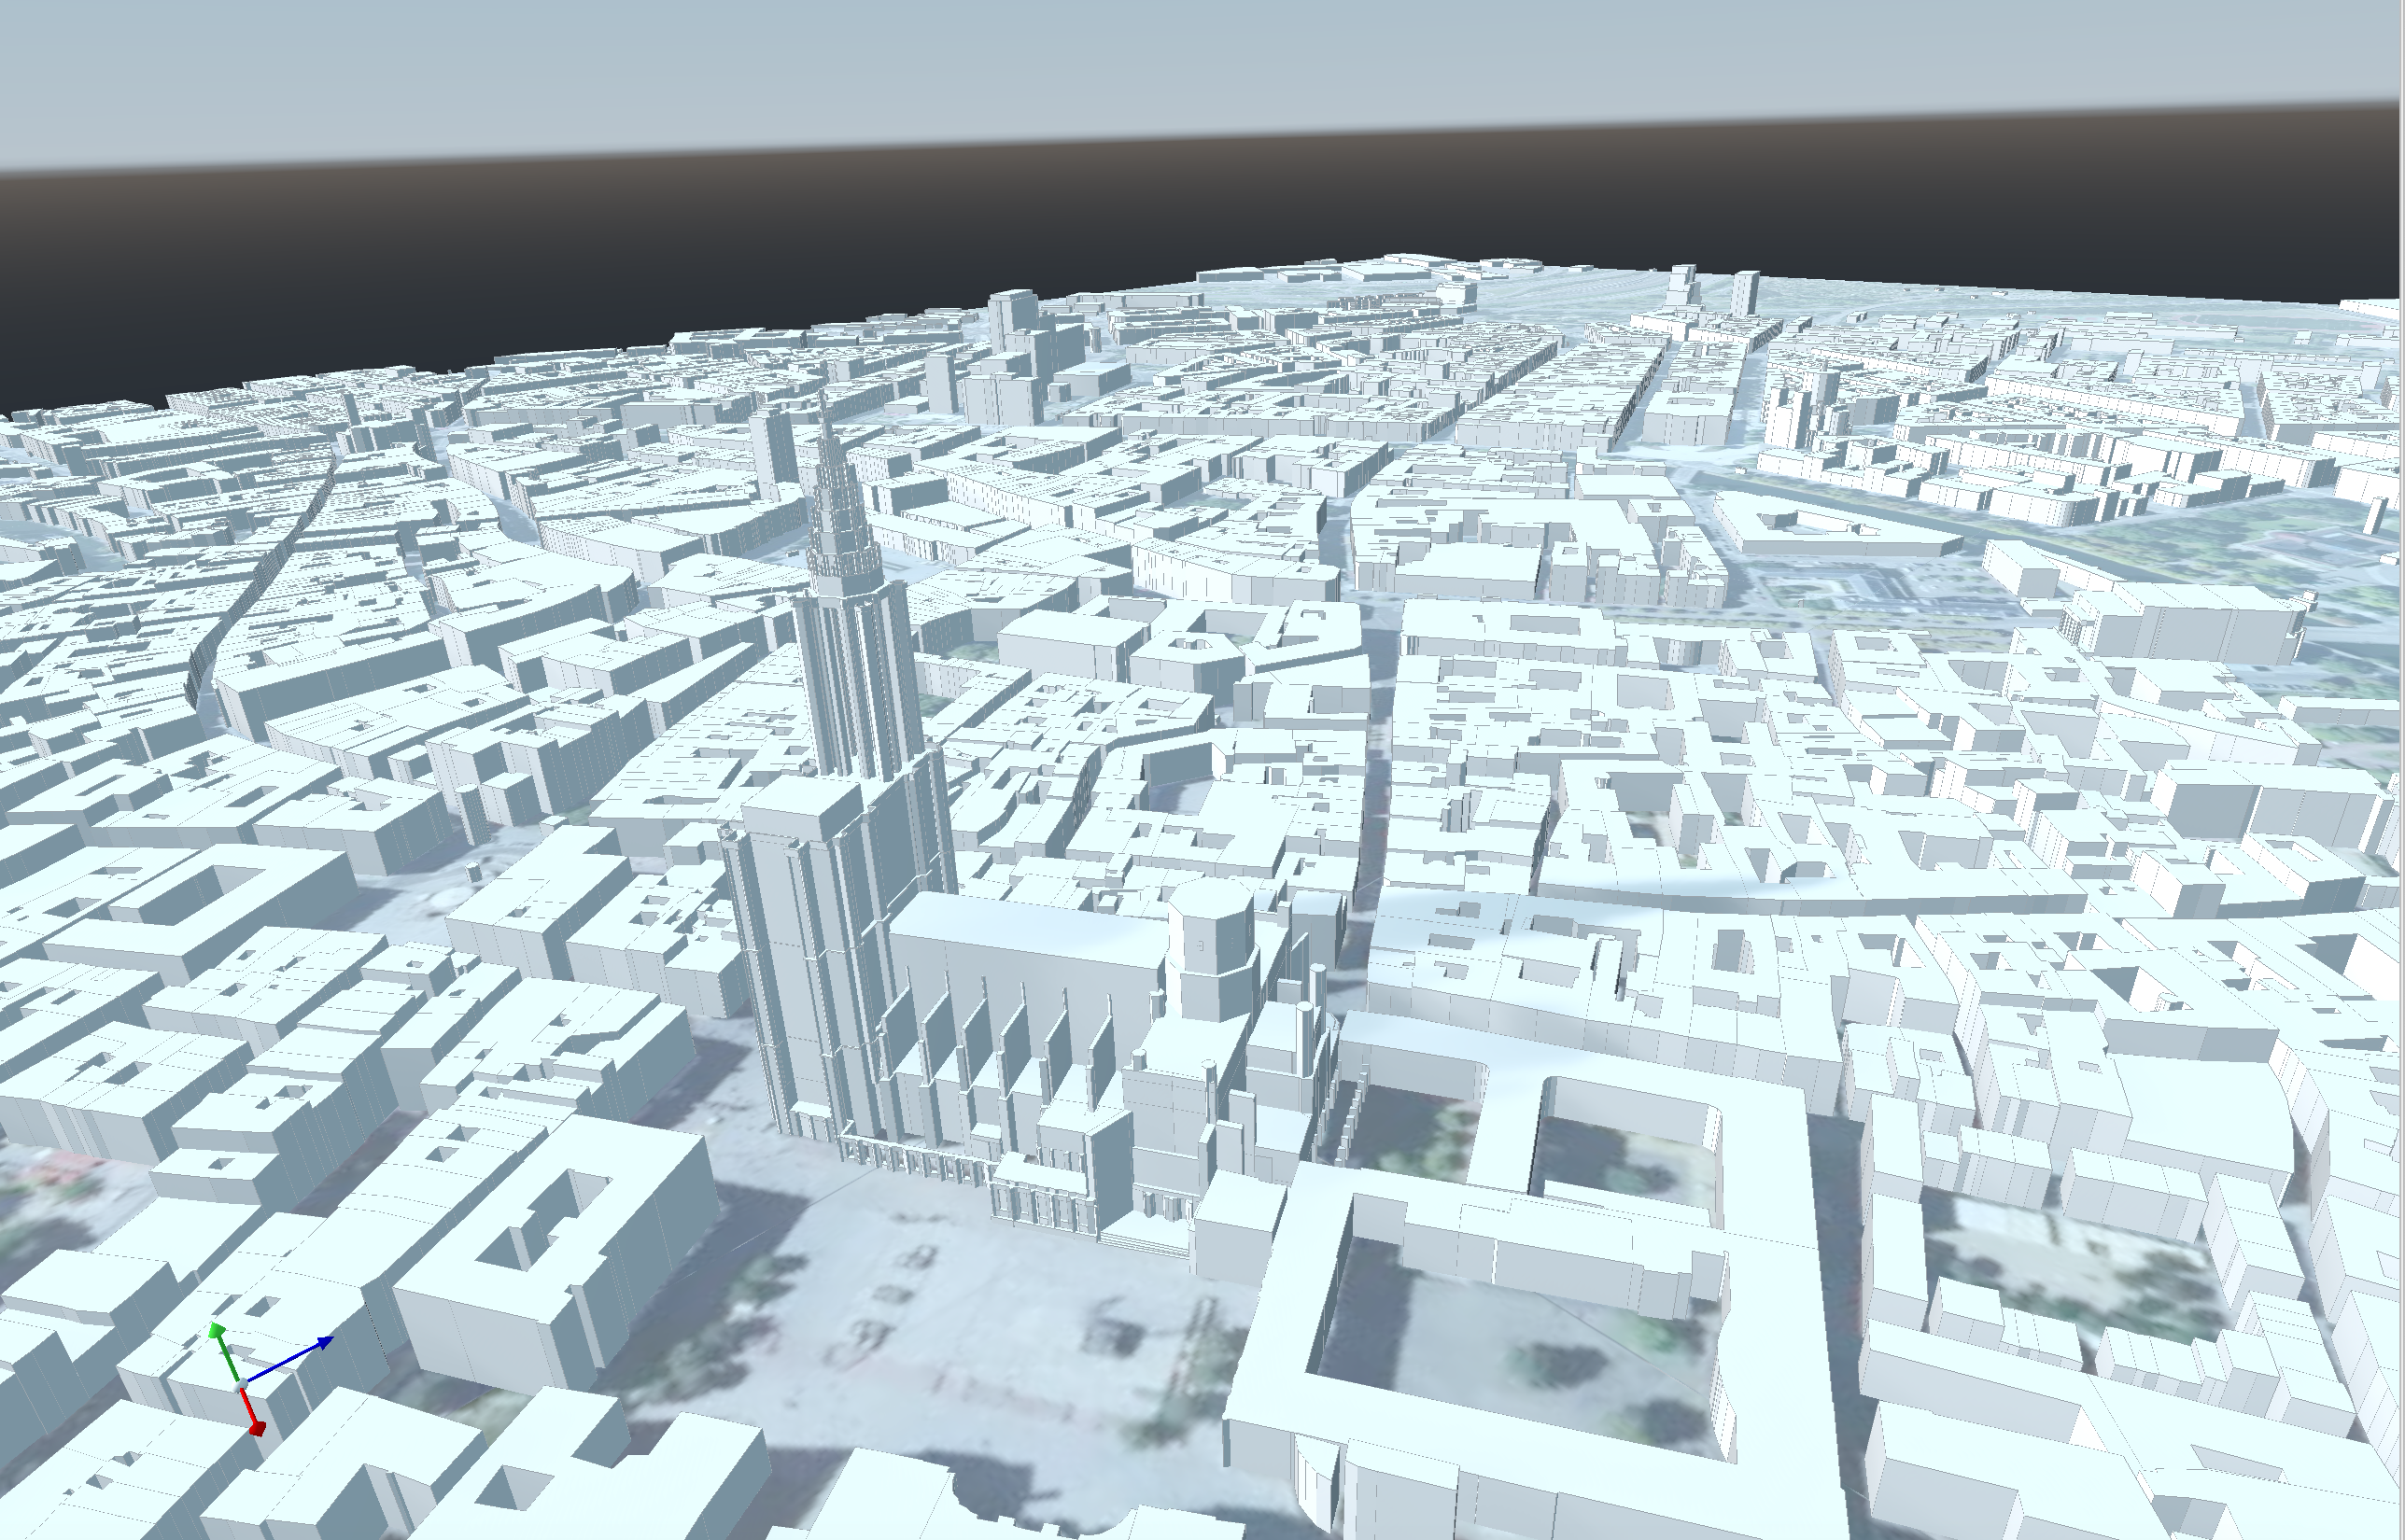
\includegraphics[width=\textwidth]{images/strasbourg-mesh-2.png}
		\caption{3D Model of Strasbourg, France}
		\label{fig:figure1}
	\end{figure}
\end{frame}

\begin{frame}{Context: Adaptibility}
	\begin{figure}
		\centering
		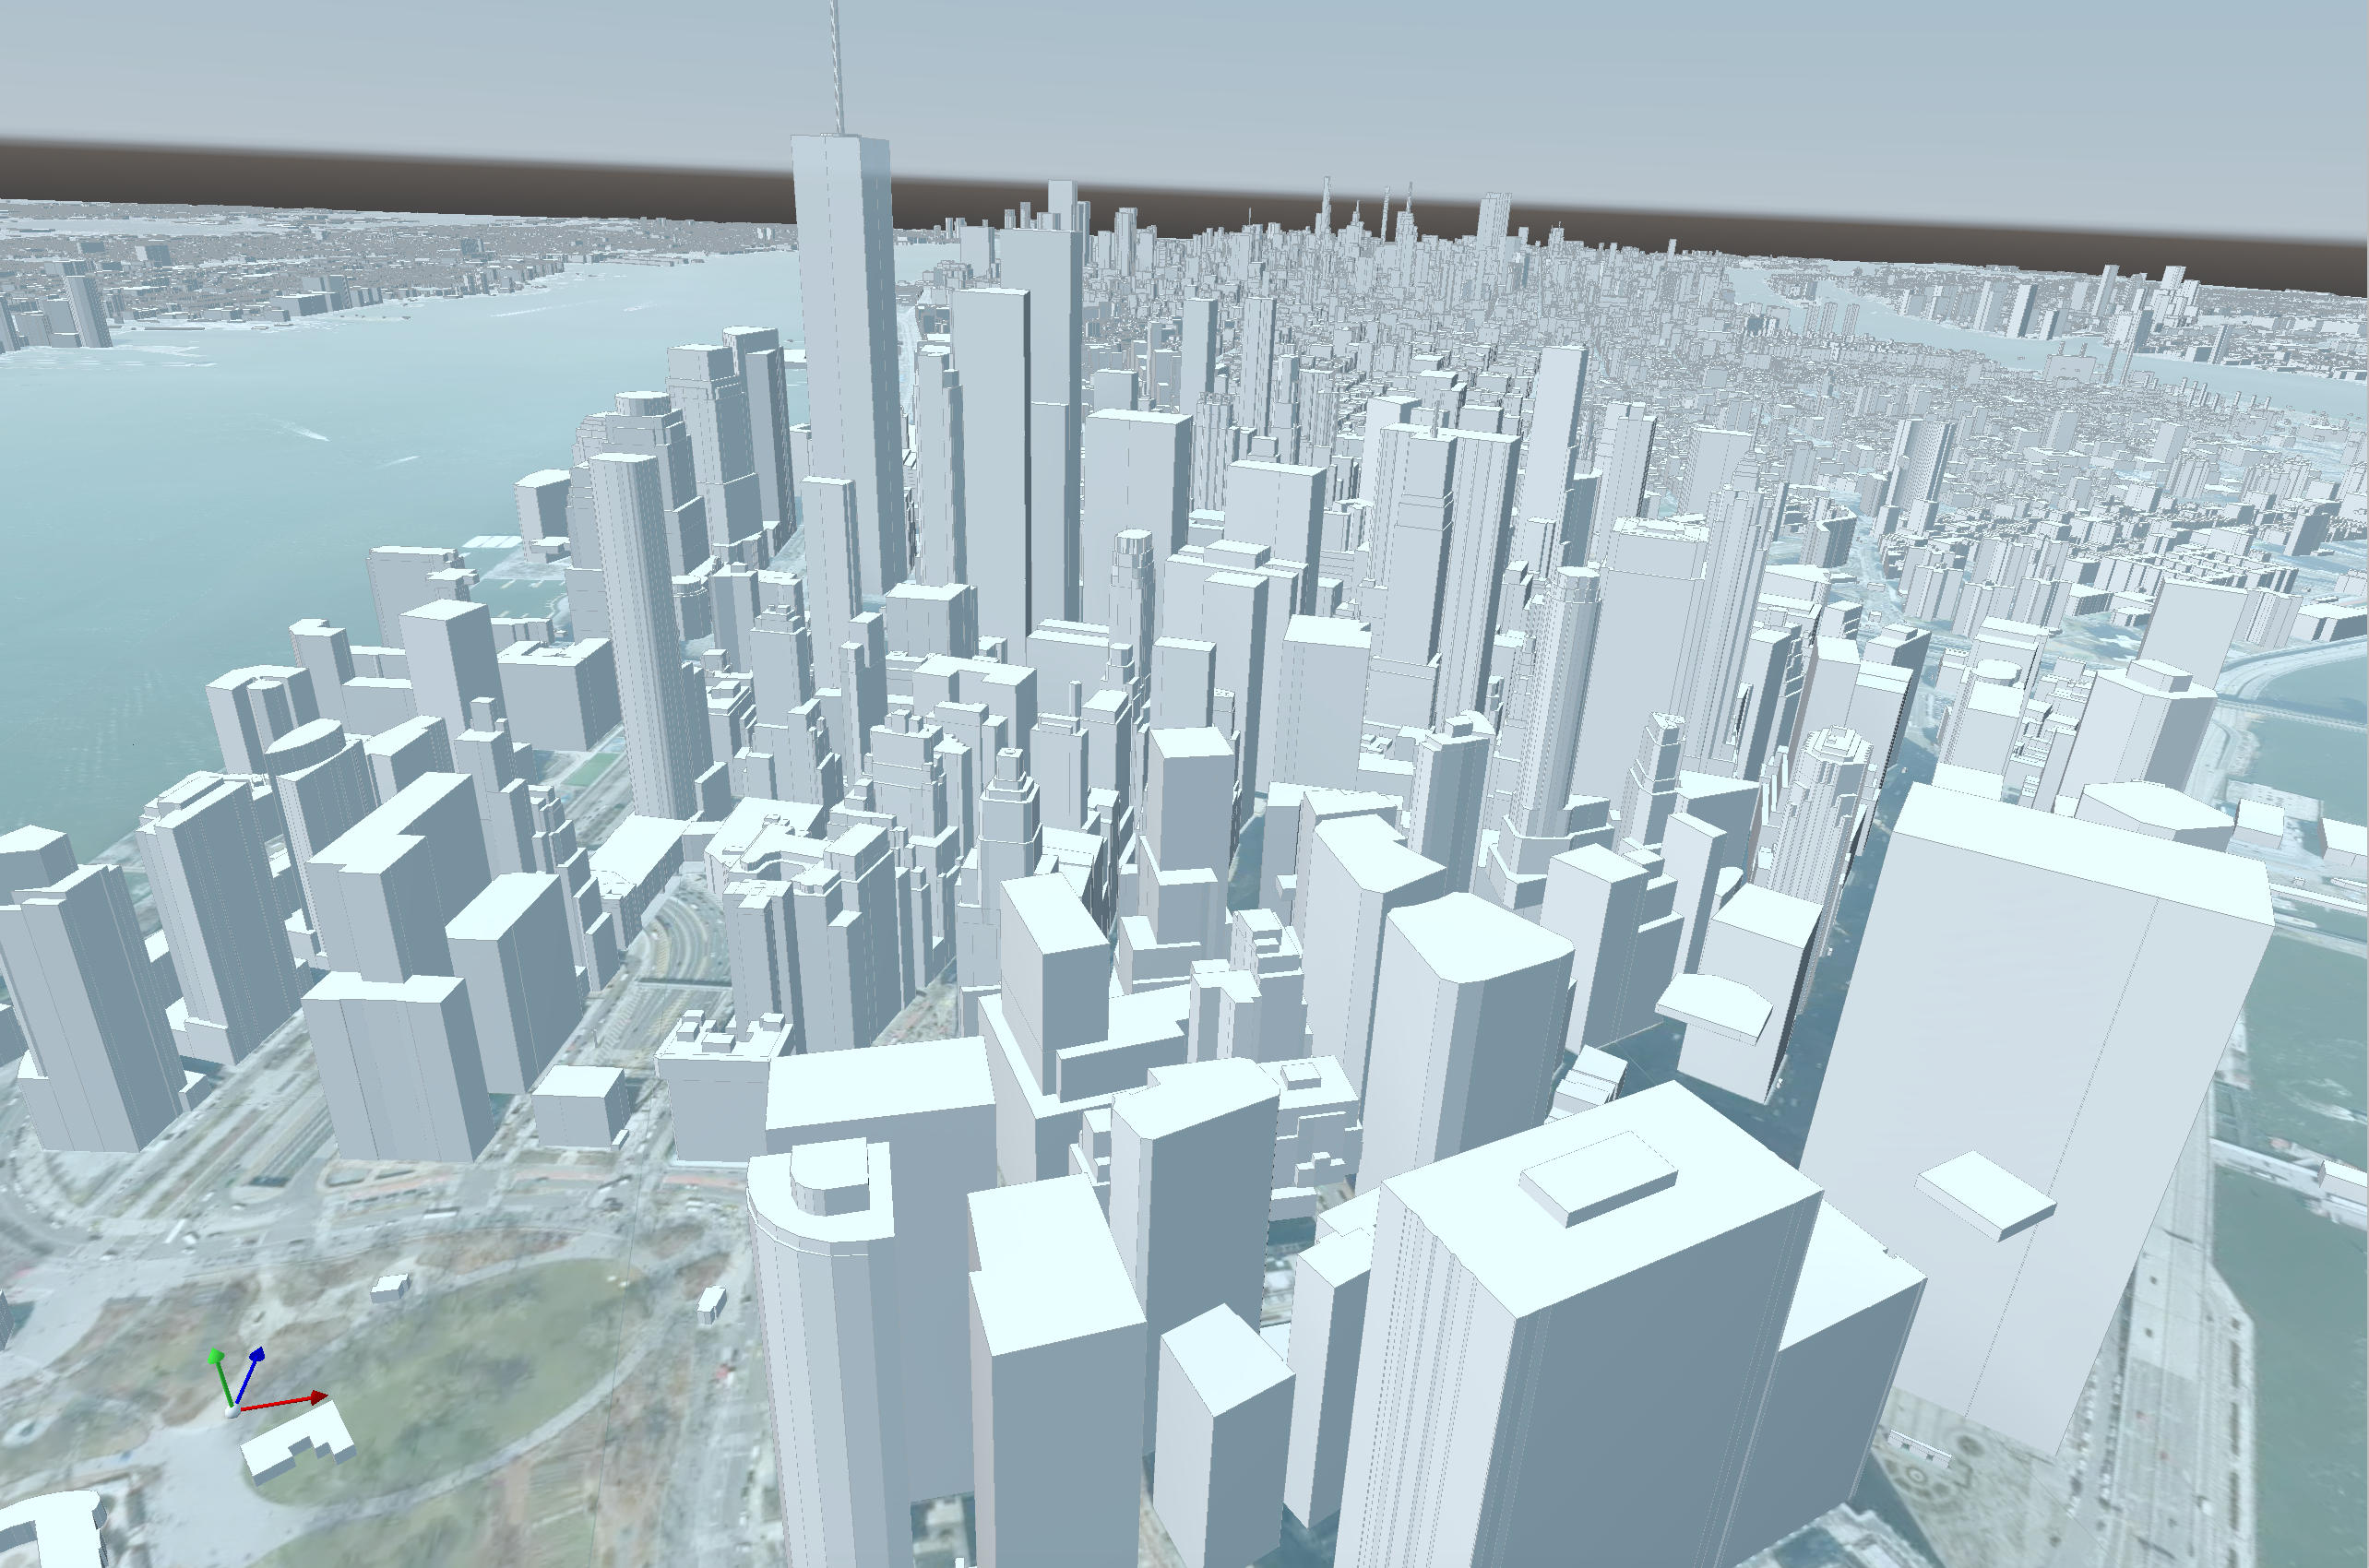
\includegraphics[width=\textwidth]{images/mesh-manhattan-2.png}
		\caption{3D Model of Manhattan, New York}
		\label{fig:figure1}
	\end{figure}
\end{frame}

\begin{frame}{Objectives}
	\Large
	\begin{itemize}
		\item \textbf{\textcolor{red}{Extracting}} \textbf{tree data} from \textbf{OpenStreetMap}
		\item \textbf{\textcolor{red}{Generating}} \textbf{3D tree models} using \textbf{CGAL} and \textbf{Gmsh}
		\item \textbf{\textcolor{red}{Integrating}} \textbf{tree models} in the \textbf{terrain mesh}
		\item \textbf{\textcolor{red}{Optimizing}} \textbf{computational efficiency}
	\end{itemize}
\end{frame}

\begin{frame}{Methodology Steps}
	\Large
	\begin{itemize}
		\item Data Acquisition
		\item Generating Tree Library
		\item Scaling Trees
		\item Wrapping Trees
		\item Placing Trees
		\item Merging Meshes
		\item Parallelization
	\end{itemize}
\end{frame}

\begin{frame}{Data Acquisition}
	\begin{figure}[h]
		\centering
		\begin{minipage}{0.49\textwidth}
			\centering
			
\includegraphics[width=\textwidth]{images/logo-openstreetmap.png}
			\caption{OpenStreetMap Logo}
			\label{fig:figure1}
		\end{minipage}\hfill
		\begin{minipage}{0.49\textwidth}
			\centering
			
\includegraphics[width=\textwidth]{images/logo-curl.png}
			\caption{Curl Logo}
			\label{fig:figure2}
		\end{minipage}
		% \caption{Overall caption for both figures}
	\end{figure}
\end{frame}

\begin{frame}[fragile]{Data Acquisition: Query Class}
	\begin{lstlisting}[language=C++]
void perform_query(std::string bbox, bool verbose) {
	std::string query =
		"[out:json]; (node(" + bbox + ")[\"natural\"=\"tree\"];); out;";
	cpr::Response r = cpr::Post(
		cpr::Url{"http://overpass-api.de/api/interpreter"}, cpr::Body{query},
		cpr::Header{{"Content-Type", "application/x-www-form-urlencoded"}},
		cpr::Timeout{10000} // Set a timeout of 10 seconds
	);
}
	\end{lstlisting}
\end{frame}

\begin{frame}[fragile]{Data acquisition: .json output}
	\begin{lstlisting}[language=json]
{
  "type": "node",
  "id": 10162018740,
  "lat": 48.5850910,
  "lon": 7.7502624,
  "tags": {
	"circumference": "1.47655",
	"diameter_crown": "5",
	"genus": "Platanus",
	"height": "6",
	"leaf_cycle": "deciduous",
	"leaf_type": "broadleaved",
	"natural": "tree",
	"ref": "16401",
	"source": "data.strasbourg.eu - patrimoine_arbore",
	"source:date": "2022-01-02",
	"species": "Platanus acerifolia x",
	"species:wikidata": "Q24853030"
  }
}
	\end{lstlisting}
\end{frame}

\begin{frame}{Generating Tree Library}
	\begin{figure}
		\centering
		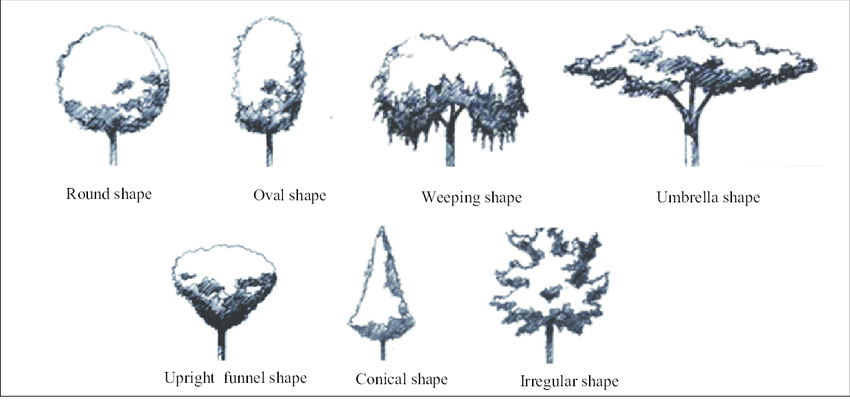
\includegraphics[width=\textwidth]{images/Different-types-of-the-trees-shape.png}
		\caption{Different tree shapes}
		\label{fig:figure1}
	\end{figure}
\end{frame}

\begin{frame}{Tree lod 0 models}
	\begin{figure}[h]
		\centering
		\begin{minipage}{0.49\textwidth}
			\centering
			
\includegraphics[width=\textwidth]{images/tree-trunk.png}
			\caption{Tree Trunk model}
			\label{fig:figure1}
		\end{minipage}\hfill
		\begin{minipage}{0.49\textwidth}
			\centering
			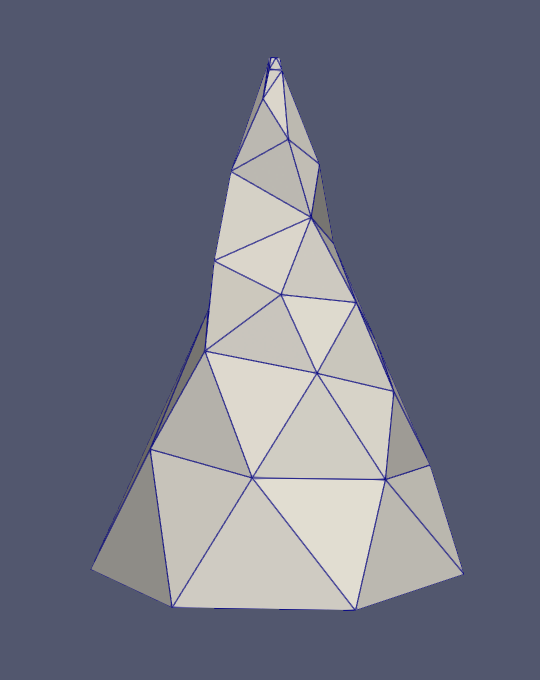
\includegraphics[width=\textwidth]{images/cone.png}
			\caption{Cone shaped Tree model}
			\label{fig:figure2}
		\end{minipage}
		% \caption{Overall caption for both figures}
	\end{figure}
\end{frame}

\begin{frame}{Tree lod 0 models}
	\begin{figure}[h]
		\centering
		\begin{minipage}{0.49\textwidth}
			\centering
			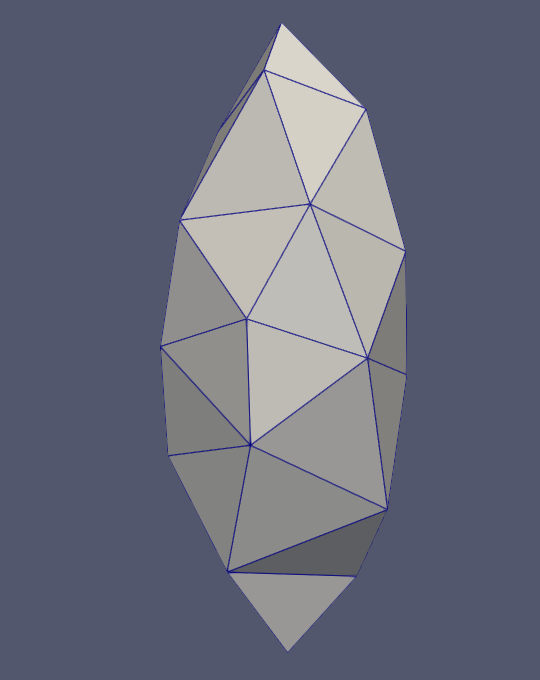
\includegraphics[width=\textwidth]{images/oval.png}
			\caption{Oval shaped Tree model}
			\label{fig:figure1}
		\end{minipage}\hfill
		\begin{minipage}{0.49\textwidth}
			\centering
			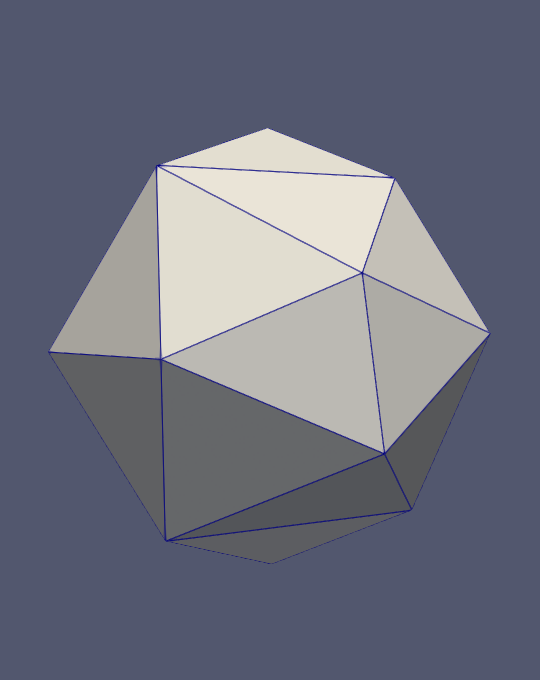
\includegraphics[width=\textwidth]{images/round.png}
			\caption{Round shaped Tree model}
			\label{fig:figure2}
		\end{minipage}
		% \caption{Overall caption for both figures}
	\end{figure}
\end{frame}

\begin{frame}{Tree lod 1,2 and 3 models}
	\begin{figure}
		\centering
		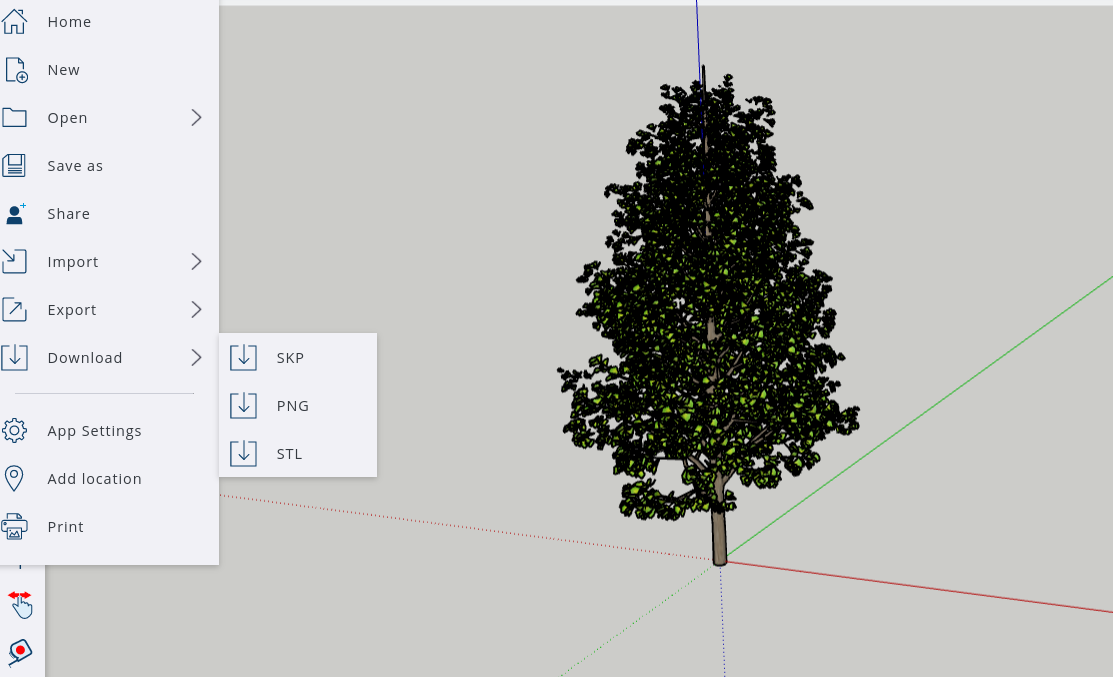
\includegraphics[width=\textwidth]{images/ginkgo-sketchup.png}
		\caption{3D model of a Ginkgo tree on Sketchup}
		\label{fig:figure1}
	\end{figure}
\end{frame}

\begin{frame}{Tree preprocessing}
	\begin{figure}[h]
		\centering
		\begin{minipage}{0.3\textwidth}
			\centering
			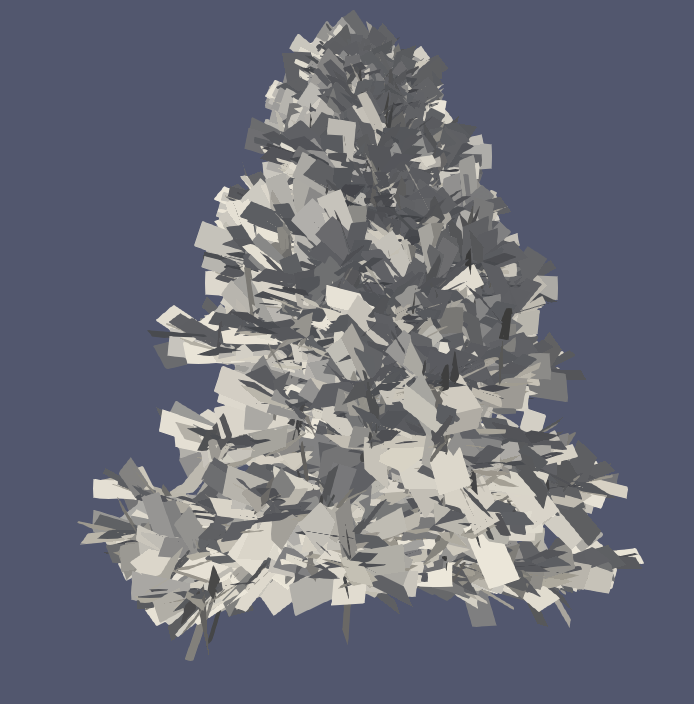
\includegraphics[width=\textwidth]{images/tree-conifer.png}
			\caption{A preprocessed conifer tree}
			\label{fig:figure1}
		\end{minipage}\hfill
		\begin{minipage}{0.3\textwidth}
			\centering
			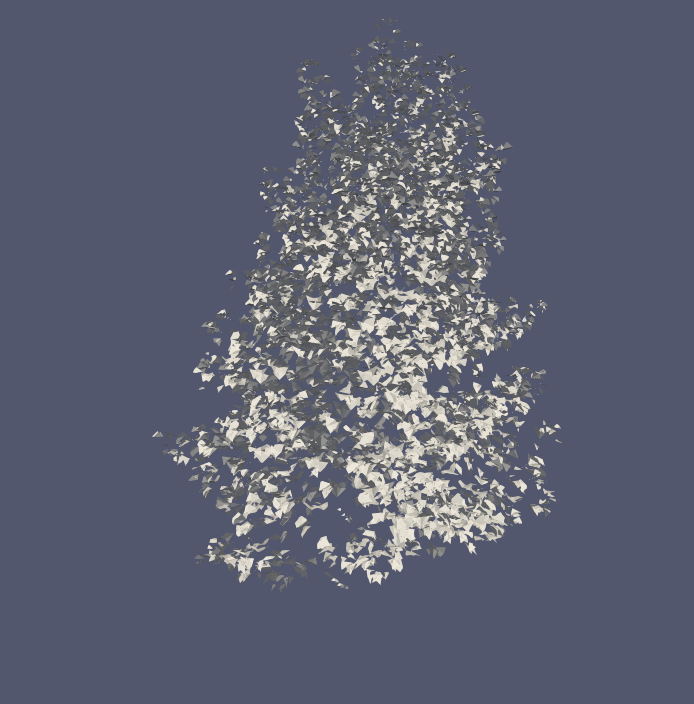
\includegraphics[width=\textwidth]{images/tree-ginkgo.png}
			\caption{A preprocessed Ginkgo tree}
			\label{fig:figure2}
		\end{minipage}
		\begin{minipage}{0.33\textwidth}
			\centering
			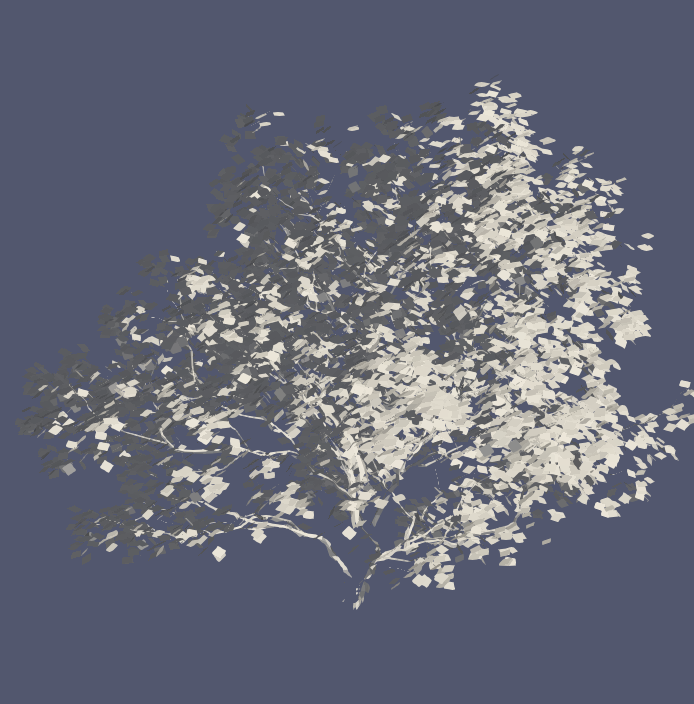
\includegraphics[width=\textwidth]{images/tree-quercus.png}
			\caption{A preprocessed Quercus tree}
			\label{fig:figure2}
		\end{minipage}
	\end{figure}
\end{frame}











\begin{frame}{Conclusion}
  \Large
  \textbf{ExaMA WP1 - Vegetation}:
  \begin{itemize}
    \item Foundation for future urban energy simulations
    integrating vegetation into the models
  \end{itemize}
\end{frame}

\begin{frame}{The end}
  \Large
  \centering
  \textbf{Thank you for your attention!}
\end{frame}

\nocite{*}
\bibliographystyle{unsrt}
\bibliography{references}

\end{document}